\input ../SlidePreamble
\input ../preamble
\usepackage{cancel}

\begin{document}

{\Huge

  \centerline{\bf TTIC 31230, Fundamentals of Deep Learning}
  \bigskip
  \centerline{David McAllester, Autumn 2023}
  \vfill
  \vfil
  \centerline{\bf Adjusting Generation}
  \vfill
  \centerline{\bf Temperature, Guidance, and Majority Voting}
  \vfill
  \vfill

\slide{Temperature-Adjusted Generation}
\begin{eqnarray*}
\mbox{Training:}\;\;\;\Phi^* & = & \argmin_\Phi E_{(x,y) \sim \pop}[-\ln P_\Phi(y|x)] \\
\\
\\
P_\Phi(y|x) & = & \softmax_y s_\Phi(y|x) \\
\\
\\
\mbox{Desired Generation:}\;\;P^\beta_\Phi(y|x) & = & \softmax_y \beta s_\Phi(y|x)\;\propto P_\Phi(y)^\beta
\end{eqnarray*}

\slide{Temperature Adjusted Generation for Language}

In practice we use

\begin{eqnarray*}
P^\beta_\Phi(y_{i+1}\;|\;y_1,\ldots,y_i) & = & \softmax_{y_{i+1}} \beta s_\Phi(y_{i+1}\;|\;y_1,\dots,y_i) \\
\\
& \propto &  P_\Phi(y_{i+1}\;|\;y_1,\ldots,y_i)^\beta
\end{eqnarray*}

\vfill
This is different from

\vfill
$$P^\beta_\Phi(y_1,\ldots,y_N) \propto P_\Phi(y_1,\ldots,y_N)^\beta$$

\slide{Temperature-Adjusted Generation for Language}

In language translation we take $\beta = \infty$ (softmax $\Rightarrow$ argmax).

\vfill
For language generation $\beta = 1$ tends to yield rambling and incoherent text.

\vfill
On the other hand $\beta = \infty$ generates repetition.

\vfill
We look for a Goldilocks $\beta$.

\vfill
An alternative to temperature-adjusted generation is top-P sampling, also called nucleus sampling, which is similar in structure and performance.

\vfill
There is a literature on generation adjustment for language.

\slide{Temperature-Adjusted Reverse-Diffusion}

{\huge

$$z(t - \Delta t) = z(t) + \left(\frac{\hat{E}_\Phi[y|t,z(t)] - z(t)}{t}\right)\Delta t + \frac{1}{\sqrt{\beta}}\;\epsilon\sqrt{\Delta t}$$

\vfill
As with language generation, this is not the same as $P^\beta_\Phi(y) \propto P_\Phi(y)^\beta$
}

\slide{Classifier Guidance}

\centerline{Diffusion Models Beat GANs on Image Synthesis}
\centerline{Dhariwal and Nichol, May 2021}

\vfill
For {\bf class-conditional} generation of imagenet images $P(y|x)$ they train an {\bf unconditional} diffusion image model $P_\Phi(y)$
and utilize a pretrained imagenet classification model $P_\Psi(x|y)$.

\vfill
\centerline{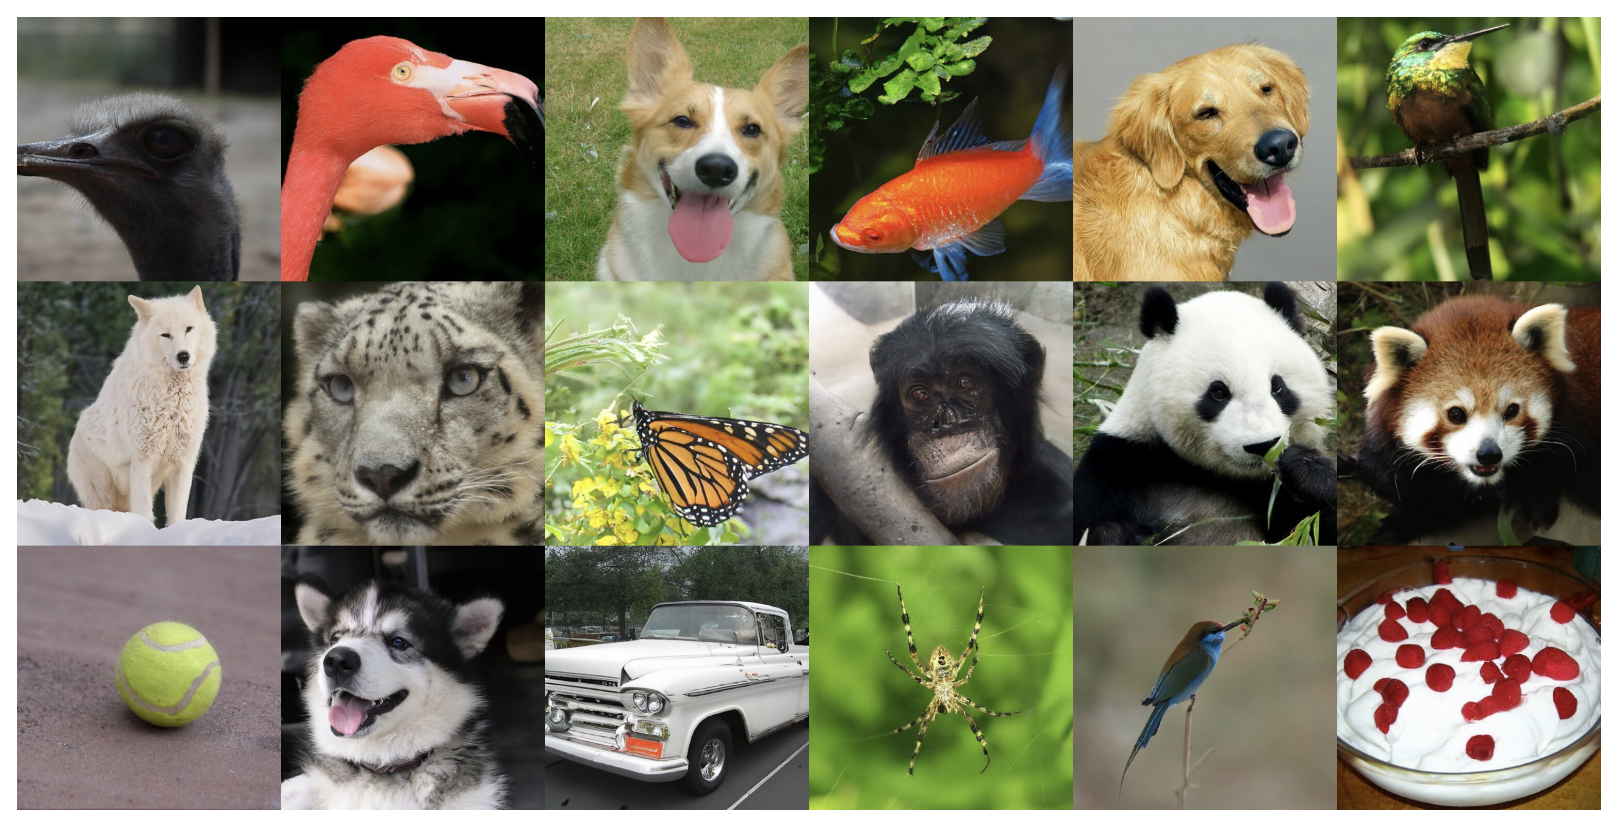
\includegraphics[width = 4in]{\images/DiffGAN}}

\slide{Classifier Guidance}

They note that

\vfill
$$P(y|x) = \frac{P(y)P(x|y)}{P(x)} \propto P(y)P(x|y)$$

\vfill
For generation they modify the reverse-diffusion process so as to intuitively approximate

$$P^{\beta,\gamma}_{\Phi,\Psi}(y|x) = \softmax_y \beta(s_\Phi(y)+ \gamma s_\Psi(x|y)) \; \propto \;P_\Phi(y)^\beta P_\Psi(x|y)^{\beta + \gamma}$$

\slide{Classifier Guidance}

{\huge $$z(t - \Delta t) = z(t) + \left(\frac{\hat{E}_\Phi[y|t,z(t)] - z(t)}{t} + {\color{red} \gamma} \nabla_z\;s_\Psi(x|z(t))\right)\Delta t
+ \frac{1}{\sqrt{\color{red} \beta}}\;\epsilon\sqrt{\Delta t}$$}

\vfill
This is different from, but motivated by,

\vfill
$$P^{\beta,\gamma}_{\Phi,\Psi}(y|x) \propto P_\Phi(y)^\beta P_\Psi(x|y)^{\beta + \gamma}$$

\slide{Conditional Diffusion Models}

$$P_\Phi(y\;|\;\mbox{panda bear chemist})$$

\vfill
\centerline{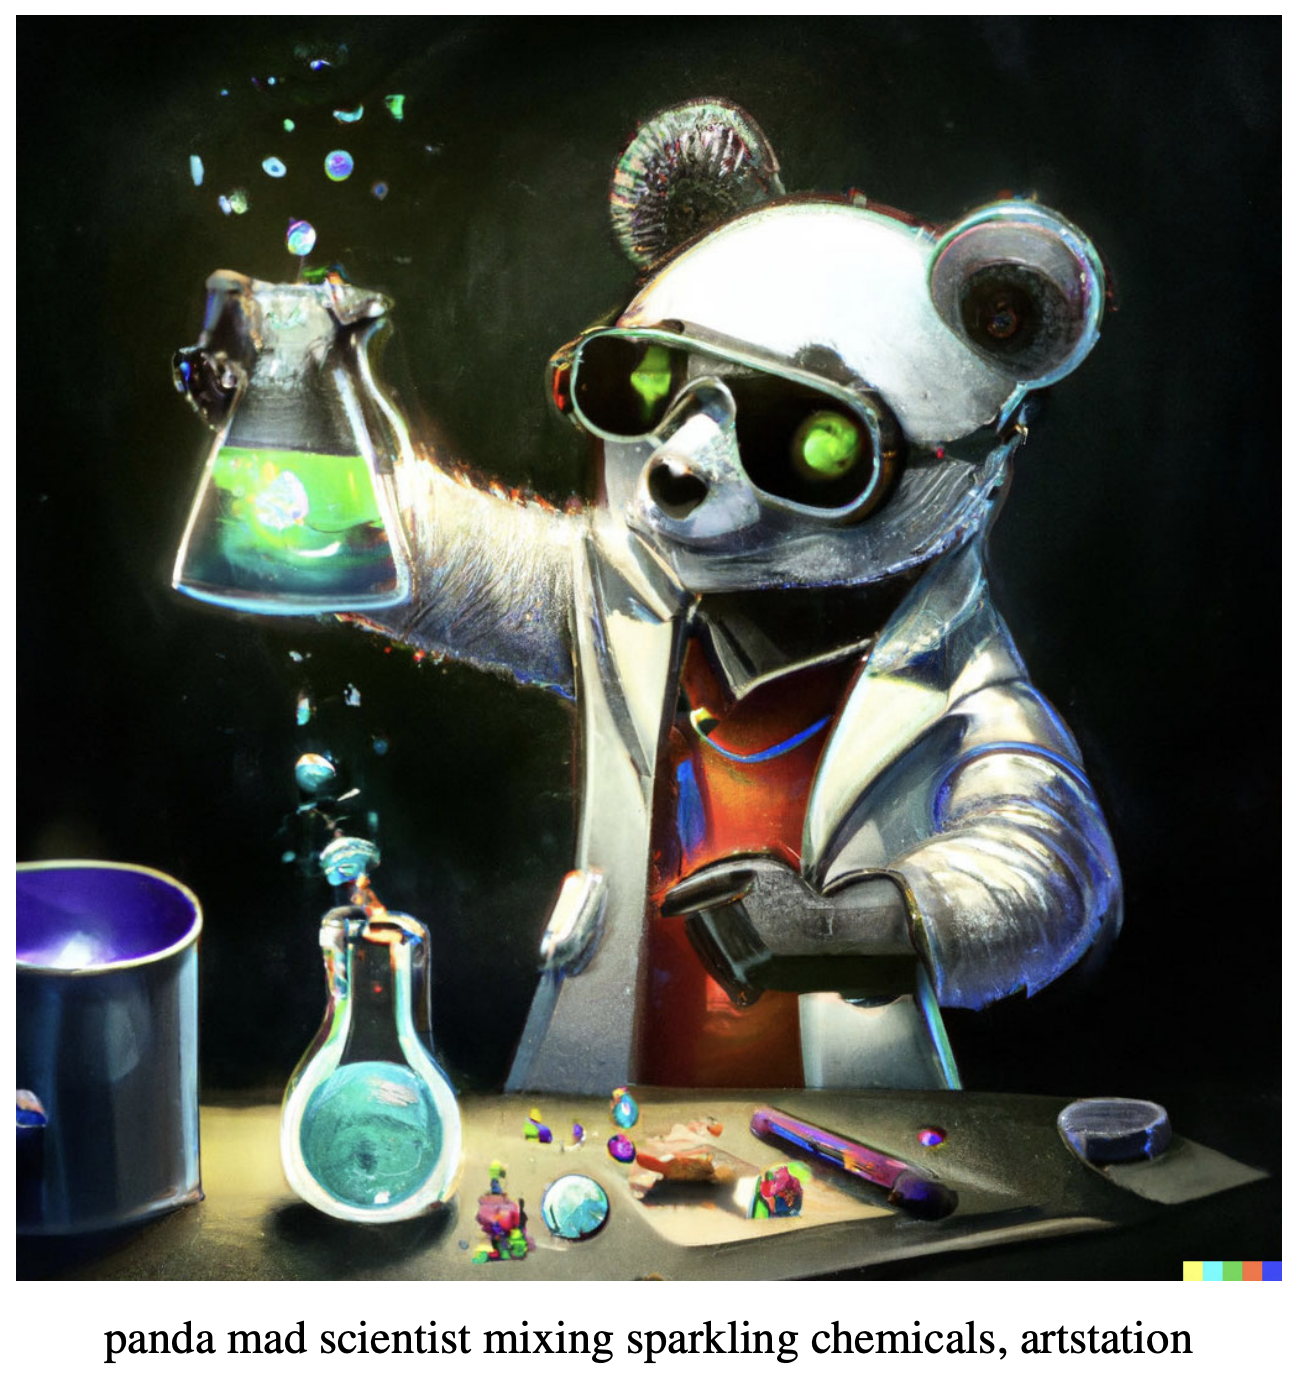
\includegraphics[width = 2.5 in]{\images/DALLEpanda}}

\vfill
\centerline {Train $\hat{E}_\Phi[y|t,z(t),{\color{red} x}]$}

\slide{Classifier Free Guidance (Self-Guidance)}

\centerline{Classifier Free Diffusion Guidance}
\centerline{Ho and Salimans, December 2021 (NeurIPS workshop)}
\begin{eqnarray*}
\mbox{Training:}\;\;\;\Phi^* & = & \argmin_\Phi E_{(x,y) \sim \pop}[-\ln P_\Phi(y|x)] \\
\\
P_\Phi(y|x) & = & \softmax_y s_\Phi(y|x)
\end{eqnarray*}

\vfill
We introduce a special $x$-value $\emptyset$ and arrange that

\vfill
{\color{red} $$\pop(y|\emptyset) = \pop(y).$$}

\slide{Guidance}

For $\beta > 0$ they modify the reverse-diffusion process to intuitively approximate
$$P^\beta_\Phi(y|{\color{red} x}) = \softmax_y  \beta s_\Phi(y|{\color{red} x}) - (\beta-1)s_\Phi(y|{\color{red} \emptyset}) \;\;\propto
\frac{P_\Phi(y|{\color{red} x})^\beta}{P_\Phi(y|{\color{red} \emptyset})^{\beta-1}}$$

\vfill
For $\beta = 1$ we have no adjustment.

$$P^1_\Phi(y|x) = P_\Phi(y|x)$$

\vfill
For $\beta >> 1$ (used in practice) we have.

$$P^\beta_\Phi(y|{\color{red} x}) \approx \softmax_y \beta(s_\Phi(y|{\color{red} x}) - s_\Phi(y|{\color{red} \emptyset})) \;\propto\; \left(\frac{P_\Phi(y|{\color{red} x})}{P_\Phi(y|{\color{red} \emptyset})}\right)^\beta$$

\slide{Guidance}


$$P^\beta_\Phi(y|{\color{red} x}) = \softmax_y \beta(s_\Phi(y|{\color{red} x}) - s_\Phi(y|{\color{red} \emptyset}))\;\;\propto \;\;      \left(\frac{P_\Phi(y|{\color{red} x})}{P_\Phi(y|{\color{red} \emptyset})}\right)^\beta$$

\vfill

\vfill
{\huge $$z(t - \Delta t) = z(t) + \left(\frac{(\hat{E}_\Phi[y|t,z(t),{\color{red} x}] - \hat{E}_\Phi[y|t,z(t),{\color{red} \emptyset}]) - z_t}{t}\right)\Delta t
+ \frac{1}{\sqrt{\beta}}\;\epsilon\sqrt{\Delta t}$$}

\slide{Guidance}

$$P^\beta_\Phi(y|{\color{red} x}) \;\;\propto \;\;  \left(\frac{P_\Phi(y|{\color{red} x})}{P_\Phi(y|{\color{red} \emptyset})}\right)^\beta$$

\vfill
Ho and Salimans motivate this from Classifier Guidance and

\vfill
{\huge \begin{eqnarray*}
P(x|y) & \propto & \frac{P(y|x)}{P(y)}
\end{eqnarray*}}

\vfill
But this is false.

\vfill
{\huge $$P(x|y) = \frac{P(x)P(y|x)}{P(y)} \;\cancel{\propto}\;\frac{P(y|x)}{P(y)}$$}

\slide{Guidance}

{\huge $$z(t - \Delta t) = z(t) + \left(\frac{(\hat{E}_\Phi[y|t,z(t),{\color{red} x}] - \hat{E}_\Phi[y|t,z(t),{\color{red} \mathrm{blurry}}]) - z_t}{t}\right)\Delta t
+ \frac{1}{\sqrt{\beta}}\;\epsilon\sqrt{\Delta t}$$}

\vfill
This will make the generated image sharper.

\slide{Conditional Generation}

Training the encoder and the decoder conditioned on $x$ (as in a language translation model).
This trains $\hat{z}_{i-1}(z_i,x)$.

\vfill
For generation we then have

{\huge
\begin{eqnarray*}
\mbox{Unadjusted:} \;z_{i-1} & = & \hat{z}_{i-1}(z_i,x) + \epsilon \\
\\
\mbox{Temperature Adjusted:}\;\;z_{i-1} & = & \hat{z}_{i-1}(z_i,x) + \frac{1}{\sqrt{\beta}}\;\epsilon \\
\\
\mbox{Guidance Adjusted:} \;\;z_{i-1} & = & \hat{z}_{i-1}(z_i,x_\mathrm{good}) - \hat{z}_{i-1}(z_i,x_\mathrm{bad}) + \frac{1}{\sqrt{\beta}}\;\epsilon
\end{eqnarray*}
}

\vfill
Output $z_1$

\slide{Adjusted Generation: Majority Voting}
\newcommand{\answer}{\mathrm{answer}}
\newcommand{\thought}{\mathrm{thought}}
\newcommand{\question}{\mathrm{question}}
\newcommand{\LLM}{\mathrm{LLM}}

{\huge
\centerline{Self-Consistency Improves Chain Of Thought Reasoning In Language Models}
\centerline{Wang et al., March 2023}
}
\vfill
The answer is taken to be a majority vote over stochastic chain of thought generation.

\begin{eqnarray*}
\answer^*(\question) 
& = & \argmax_{\answer}\\
\\
& & \;\;\;\;E_{\thought \sim P_{\LLM}({\thought|\question})} \\
\\
& & \;\;\;\;\;\;\;\;P_\LLM(\answer|\question;\thought)
\end{eqnarray*}


\slide{END}
}
\end{document}

